\usepackage{tikz}

% Aquí van todas las figuras en TikZ

\newcommand{\esquemavm}{
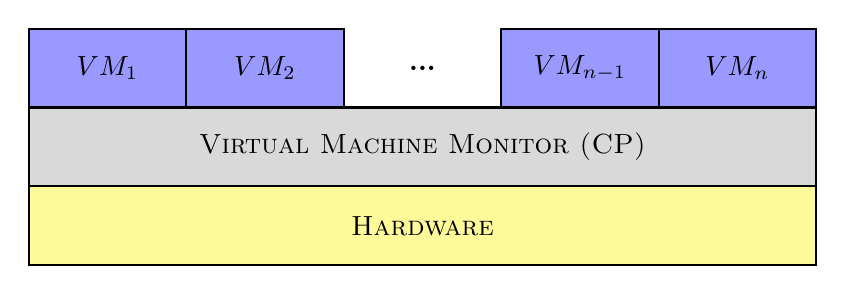
\begin{tikzpicture}
	\draw[fill=blue!40, thick] (0,2) rectangle (2,3);
	\draw[fill=blue!40, thick] (2,2) rectangle (4,3);
	\draw[fill=blue!40, thick] (6,2) rectangle (8,3);
	\draw[fill=blue!40, thick] (8,2) rectangle (10,3);
	\draw[fill={gray!30}, thick] (0,1) rectangle (10,2); 
	\draw[fill=yellow!40, thick] (0,0) rectangle (10,1); 
	
	\node at (1,2.5) {$VM_1$};
	\node at (3,2.5) {$VM_2$};
	\node at (5,2.5) {\textbf{...}};
	\node at (7,2.5) {$VM_{n-1}$};
	\node at (9,2.5) {$VM_n$};
	\node at (5,1.5) {\textsc{Virtual Machine Monitor (CP)}};
	\node at (5,0.5) {\textsc{Hardware}};
\end{tikzpicture}
}
